\documentclass[../../Aurora C# unofficial manual.tex]{subfiles}

\begin{document}
	\section{Ground support fighters}
	Original post can be found
	\href{http://aurora2.pentarch.org/index.php?topic=8495.msg109886#msg109886}{here}.
	\\\\
	
	Fighters equipped with fighter pods can provide support to ground unit formations during ground combat.
	
	To be eligible, a fleet with fighters is given an order to "Provide Ground Support" with a friendly population as the destination. This order functions in a similar way to a 'Follow' order, with the order remaining in place until removed by the player. On the Ground Combat Window, eligible fleets appear in their own section for each population. These fleets can be dragged and dropped on to formations in the same way as superior and subordinate formations. Fleets with this order that are at their target population cannot be targeted in normal naval combat or by STO weapons.
	
	In combat, the ground support fighters attack at the same time as bombardment elements and have the same target selection options as heavy bombardment.
	
	Ground support fighters have the same chance to hit as ground units, although they are not affected by any negative environmental modifiers (such as high gravity or extreme temperatures). Each fighter's to hit chance is affected by its own crew grade and morale.
	
	Each Forward Fire Direction component in a formation allows support from up to six ground support fighters. If more fighters are assigned to a formation than can be supported, the chance to hit is modified by \( Number Of FFD * 6 / Number Of Fighters \).
	\begin{figure}[H]
		\centering
		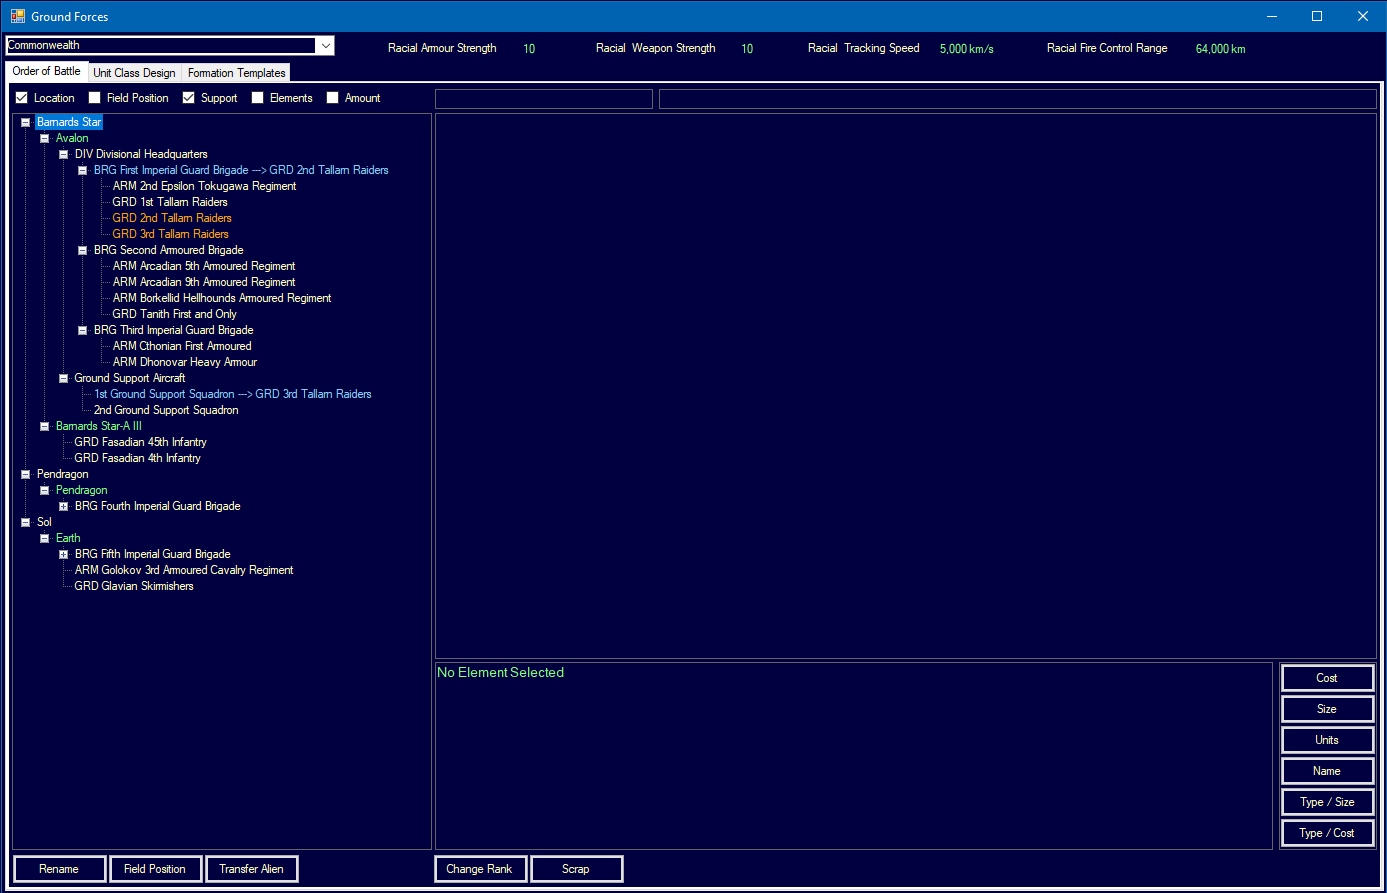
\includegraphics[width=0.95\linewidth]{images/GroundSupportFighters}
		\caption[Ground Support Fighters]{Ground Support Fighters Example}
		\label{fig:groundsupportfighters}
	\end{figure}
\end{document}